%Preamble--------
\documentclass[a4paper, 12pt]{article}
%Package_List ------------
\usepackage{fancyhdr}
\usepackage[a4paper,left=30mm,right=30mm,top=15mm,bottom=22mm]{geometry}
\usepackage{float}
\usepackage{graphicx}
\usepackage{amsmath, amsfonts, amssymb}
\usepackage{mathptmx}
\usepackage[nottoc, notlot, notlof]{tocbibind}
\usepackage{tabularx}
\usepackage{titlesec}
\usepackage{enumitem}
\usepackage{multicol}
\usepackage[backend=bibtex,style=ieee,sorting=none]{biblatex}
\addbibresource{ref.bib}

%End Package_List ----------
\titleformat*{\section}{\huge\bfseries}
\titleformat*{\subsection}{\large\bfseries}
\titleformat*{\subsubsection}{\large\bfseries}
\titleformat*{\paragraph}{\normalsize\bfseries}
\titleformat*{\subparagraph}{\normalsize\bfseries}
\graphicspath{{./images/}}
\setlength{\headheight}{15pt}
\pagestyle{fancy}
\fancyhead{}
\fancyfoot{}
\fancyhead[L]{\textbf{\leftmark}}
\fancyfoot[C]{\thepage}
\setlength{\parindent}{0ex}
\setlength{\parskip}{1.5em}
\linespread{1.3}
\title{Hindi Tweets Sentiment Analysis Using Transfer Learning}
%\subtitle{Abstract}
\author{Anubhav Mehra}
\date{\today}

%End Preamble -------------


\begin{document}
\begin{titlepage}
	\begin{center}
		\vspace*{1cm}
			\Large{\textbf{Hindi Tweets Sentiment Analysis Using Transfer Learning}}\\
			\vspace*{3cm}
			\large{\textbf{Pre Ph.D. DISSERTATION}}\\
			\vspace*{3cm}
			\large{\textit{\textbf{by}}} \\
			\vspace*{3cm}
			\large{\textbf{Anubhav Mehra}}\\
			\vfill
			\Large{\textbf{DEPARTMENT OF COMPUTER SCIENCE \\ S.S.J. UNIVERSITY ALMORA \\ ALMORA - 263601(INDIA) \\ JULY, 2021}}
			
			\normalsize
			
	\end{center}
\end{titlepage}
\begin{sloppypar}
\begin{center}
\textbf{\underline{ACKNOWLEDGMENT}}
\end{center}
It is a genuine pleasure to express my deep sense of gratitude to my mentor and my Ph.D. supervisor Dr. Manoj Singh Bisht. His advice and approach have helped me to a very great extent to accomplish this task. 

I would also like to extend my gratitude to the Department of Computer Science, S.S.J University, Almora and all its faculty members who have been of great help during the course of this project.

Finally I would like to thanks my head Dr. Ashish Mehta, Department of Computer Science, DSB Campus Nainital for his immense help and providing me with time to complete my dissertation work.
\thispagestyle{empty}
\clearpage
\begin{center}
\textbf{\underline{DECLARATION}}
\end{center}
I declare that this written submission represents my ideas in my own words and where others' ideas or words have been included, I have adequately cited and referenced the original sources. I also declare that I have adhered to all the principles of academic honesty and integrity and have not  misrepresented or fabricated or falsified any idea/data/fact/source in my submission. I understand that any violation of the above will be cause of disciplinary action by the University and can also evoke penal action from the sources which have thus not been properly cited or from whom proper permission has not been taken when needed.
\begin{flushright}
Anubhav Mehra \\
\today
\end{flushright}
\thispagestyle{empty}
\clearpage
\begin{center}
\textbf{\underline{ABSTRACT}} \\ [0.5ex]
\end{center}
 Sentiment analysis is a \textbf{natural language processing} technique to find if the sentiment of the text is positive, neutral or negative. Traditionally, to train a model for sentiment analysis require very dense neural networks to train on very huge datasets. But, here we have used a technique called \textbf{Transfer Learning} that stores a model which has learned some knowledge, that we can leverage in solving some other tasks based on the knowledge of the previous model. Here we are using a language model called  \textbf{BERT(Bidirectional Encoder Representations from Transformers)}. BERT is a pertained model which learns using the learning techniques developed by Google. The BERT multilingual base model that we are using is pertained on the top 104 languages including Hindi. We then leverage the power of this model for the Sentiment analysis of the Hindi texts dataset that we've got. This allows us to achieve moderately high accuracy scores using a comparatively small dataset.

\textbf{Keywords:} Sentiment Analysis, Emotion AI,  Natural Language Processing, Transfer Learning, BERT, Multilingual Natural Language Processing, Hindi Sentiment Analysis.
\thispagestyle{empty}
\clearpage
\tableofcontents
\thispagestyle{empty}
\clearpage
\setcounter{page}{1}
\section{Introduction}

\subsection{Transfer Learning}
Transfer Learning is a Machine Learning method where a model that is trained for a certain task is utilized as the starting point for solving some other task i.e., to train a second model from the knowledge learned from the first model as well as the dataset. It is a very popular approach in natural language processing domain to solve problems such as getting the context of the text.

\begin{figure}[H]
\begin{center}
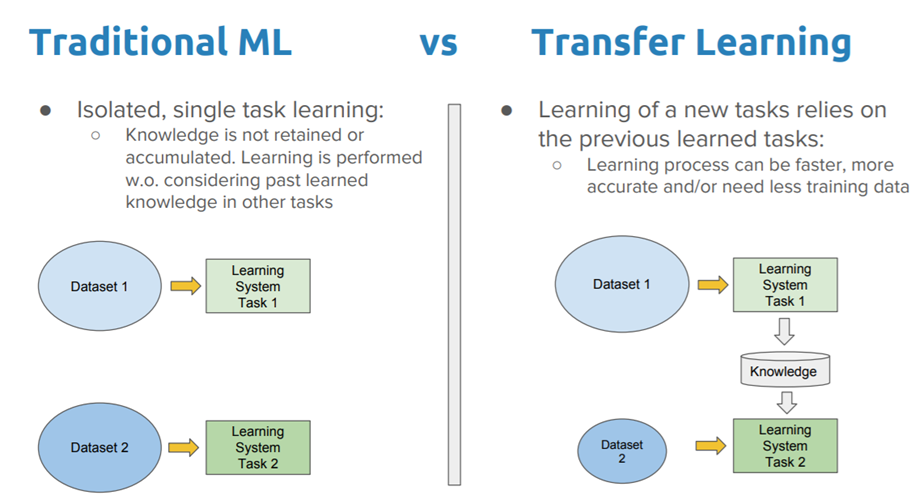
\includegraphics[scale=0.45]{tl.png}
\caption{Differentiation between Traditional and Transfer Learning Methodology. \label{tl}} %cite here guide to tl 
\end{center}
\end{figure}

The inspiration for transfer learning comes from us - humans, ourselves - where in, we have an inherent ability to not learn everything from scratch. We transfer and leverage our knowledge from what we have learn in the past for tackling a wide variety of tasks.\cite{sarkar_deep_2018}

\large \textbf{Deciding when to use Transfer Learning} \\ [0.5ex]
\normalsize
As with any technique at our disposal we must have a very clear reason on using transfer learning. First and foremost, we must realize that we can't use transfer learning in every situation. This is because for transfer learning to work we must have a model trained on a similar task. As with the problem concerned in our dissertation here, we have  a language model available which is trained in recognizing linguistic structure of  various languages. Now, we can leverage the power of this model to train a new model for our
\thispagestyle{empty}
\clearpage
 context analysis problem. If this is the case, you will realize that transfer learning is a very decent technique to use for acquiring better results and that too in very short amount of time than traditional methods. Now, with this out of the way you may want to use transfer learning if you have following conditions:
\begin{itemize}
\item{You have a smaller dataset}
\item{You are constrained on time}
\end{itemize}

\large \textbf{Applications of Transfer Learning} \\ [0.5ex]
\normalsize
There are various applications of Transfer Learning in variety of domains. In \textbf{Image Recognition}, transfer learning can be used to perform various imaging tasks. For e.g.,  a model trained to identify face can be used for facial recognition. Transfer Learning can also be used in \textbf{Speech Recognition} tasks.  For e.g., a model trained in a particular language for speech recognition can be used to train a model for speech authentication. But our key domain of interest where we are most interested in using this technique is \textbf{Natural Language Processing}. Transfer learning can be used to solve various tasks in  NLP. For e.g., a model trained in recognizing the linguistic structure of a language can be used to train a model to predict next word based on the series of words it gets in the previous sentences.

\subsection{Sentiment Analysis}
One such task in NLP is \textbf{Sentiment Analysis}. Sentiment Analysis or emotion AI, is the process in natural language processing  of subjective emotional analysis of the text. Primarily sentiment analysis finds if the emotional tone of a piece of writing is \textbf{\textit{positive, neutral or negative}}. \textbf{Table \ref{table: category}} lists some examples of what a sentiment analysis categorization may look like.
\begin{table}[H]
\caption{ Sentiment Analysis Categorization.\label{table: category}}

\begin{tabularx}{\columnwidth}{| X | X |}
\hline
Text & Category \\ [0.5ex]
\hline
\hline
That restaurant has a great food & Positive \\ [0.5ex]
\hline
He is my brother's colleague & Neutral \\ [0.5ex]
\hline
Bollywood movies are not entertaining & Negative \\ [0.5ex]
\hline
\end{tabularx}
\end{table}

As we can see it is easily understood by a human brain what sentiments these pieces of writing represent. But, for a computer this is a very challenging problem. It is a challenging problem because the way humans communicate using natural languages is extremely varied depending  upon \textit{subjectivity}, \textit{use of irony}, and the \textit{context} of the phrase. Not all verbs, nouns and pronouns can be treated equally when analyzing the emotional tone of the text. The tone of our phrases depends on how we are using them, when we are using them and for what we are using them. For e.g., the phrase \textit{absolutely everything}, can be an answer to a question like \textit{What are you so happy about?} or can equally be an answer to a completely opposite  question \textit{What are you so sad about?}. Thus, the emotional tone of the phrase can have completely separate meaning depending upon the various parameters. In the example above, the context of the phrase can alter the emotional meaning of the phrase completely. 

\large \textbf{Applications of Sentiment Analysis} \\[0.5ex]
\normalsize
Listed below are some applications of Sentiment Analysis:
\begin{itemize}
\item{
\textbf{Social Media Monitoring: } Sentiment analysis is very useful tool to find out what is a general sentiment of people in social media towards a product, person, situation, trend or any such topic of interest.}
\item{
\textbf{Feedback Analysis: } Sentiment analysis can also be used to find the whether the  reception of new policies or workings of a company or of a government is positive or negative. This helps a company or government to evaluate their policies and performance using a well-defined metric.}
\item{
\textbf{Market Research: } Sentiment analysis can also be used to find what topics are viewed in positive and negative light in current landscape. This information can then be used to design or steer a companies marketing campaign to align with those sentiments.}
\end{itemize}


\begin{figure}[H]
\begin{center}
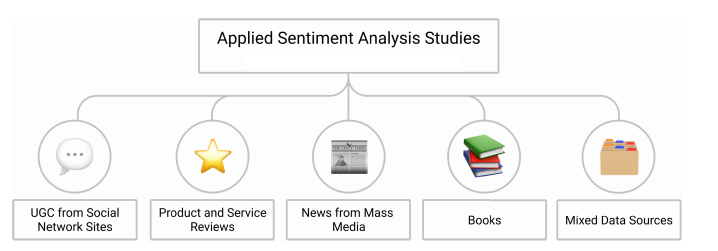
\includegraphics[scale=0.7]{cat.png}
\caption{Application of Sentiment Analysis. \label{cat}} %cite here the application of SA
\end{center}
\end{figure}

\subsection{Purpose}

The purpose of this project is to showcase the use of Transfer Learning in developing a model for Sentiment Analysis of Social Media Posts( tweets in this case) posted in Hindi Language. Thus, calculating the accuracy of the model trained on a relatively small dataset and quick training time compared to those that would have been required if we would've followed a Traditional ML route. Hence, contributing in the field of Machine Learning and Data Science for any future project work in technology development.

\subsection{Dissertation Structure}
\textbf{Chapter 2:} This chapter discusses the literature review of this project. It discusses the concepts of this project, related an similar works done.

\textbf{Chapter 3:} This section describes the steps of the method followed to complete the project, which includes data sourcing, data preprocessing, model selection, model implementation, accuracy score calculation.

\textbf{Chapter 4:} This section describes the result and conclusion of the project.

\textbf{Chapter 5:} This section details what further works and improvements can be incorporated in the project.

\textbf{Chapter 6:} This section contains the bibliography for this dissertation.
\clearpage

\section {Review of Literature}

This section details various concepts behind this project, their workings and also similar types of works that have been done.

\subsection{Concept of Transfer Learning}

\subsubsection{General Idea}
While, we have new and better techniques of developing deep neural networks that are astoundingly great at predicting outputs for particular features set. We still have a problem at hand. What our models still frightfully lack is the ability to generalize to conditions that are different from the ones encountered during training. When is this necessary? Every time you apply your model not to a carefully constructed dataset but to the real world. The real world is messy and contains an infinite number of novel scenarios, many of which your model has not encountered during training and for which it is in turn ill-prepared to make predictions. %cite ruder.io

So to make a generalizing model the dataset required that would enable the model to learn the working in the real world would be astoundingly huge. Collecting such dataset may be difficult, expensive and can also be downright impossible in many cases. So for a solution we turns our head towards transfer learning.

Humans are generally very good at transfer learning. We use our knowledge at one task to solve a related task all the time. For example, if you have any experience programming with Java, C/C++ or any other programming languages, you’re already familiar with concepts like loops, recursion, objects and etc (Figure \ref{human}, a). If you then try to pick up a new programming language like python, you don’t need to learn these concepts again, you just need to learn the corresponding syntax. Or to take another example, if you have played table tennis a lot it will help you learn tennis faster as the strategies in these games are similar (Figure \ref{human}, b). %cite medium article

\begin{figure}[H]
\begin{center}
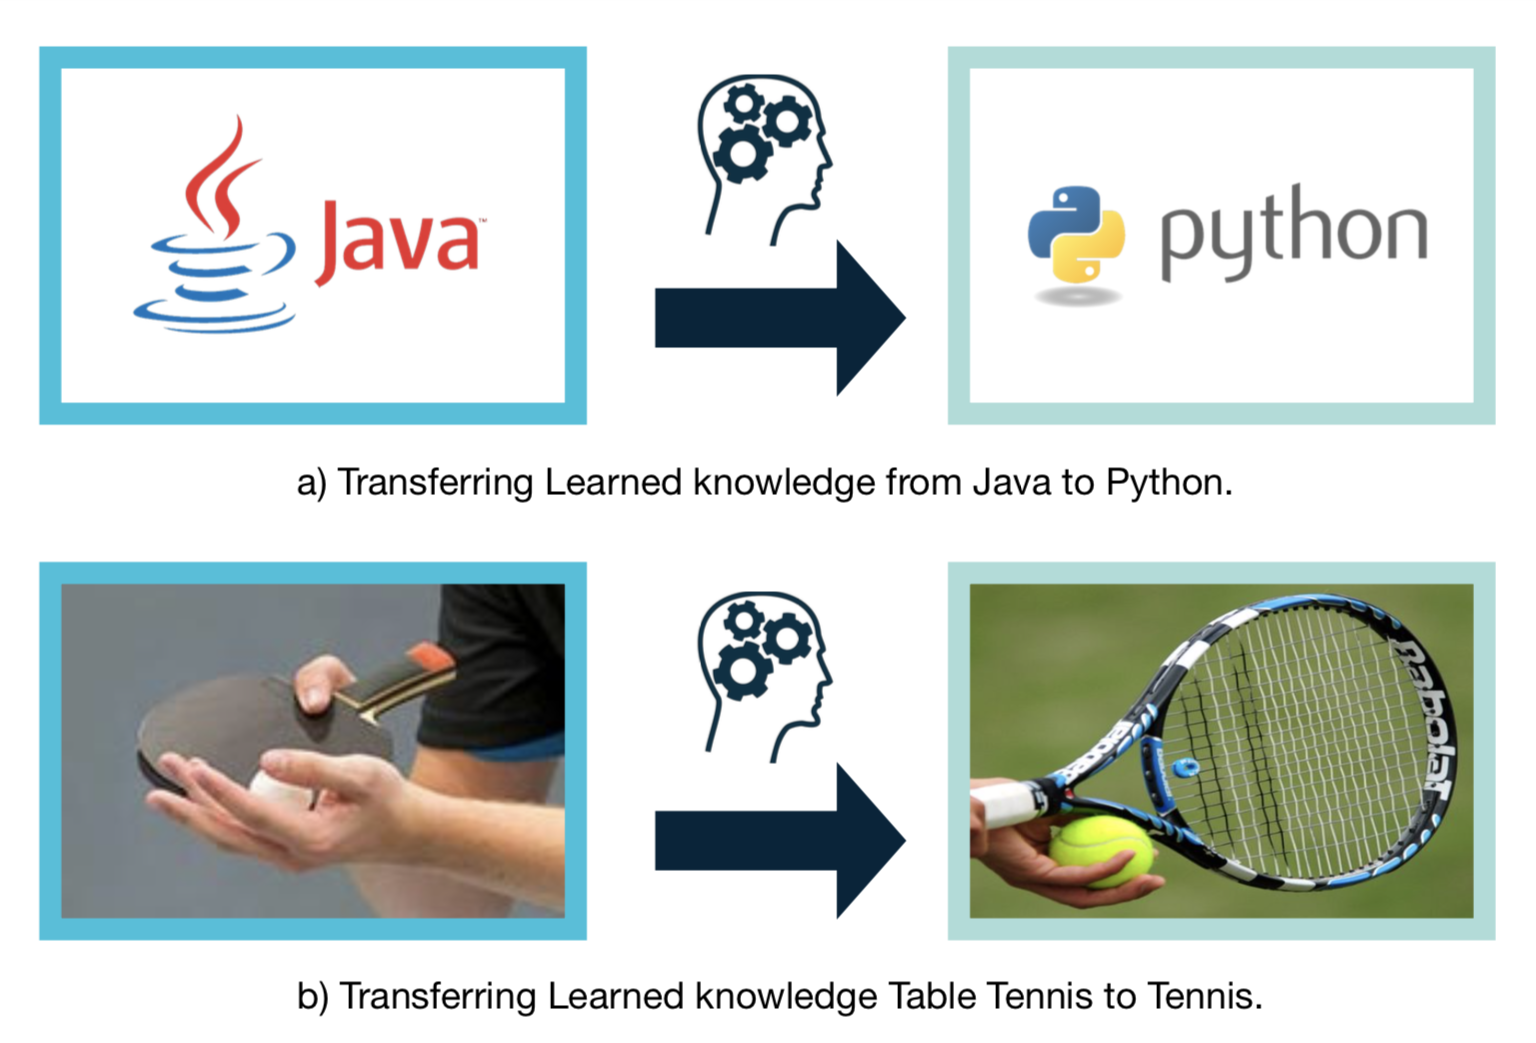
\includegraphics[scale=0.25]{human_lt.png}
\caption{Transferring the learned knowledge in humans.\label{human}} % cite medium article
\end{center}
\end{figure}

In Transfer Learning as compared to Traditional Learning  where models are trained in complete  isolation, we use the knowledge gained by a model in solving a task of similar domain to train our desired model to solve some other task.

\subsubsection{Definition of Transfer Learning}

Following is the definition of Transfer Learning in terms of domain and tasks.

A domain $D$ consists of: a feature space $X$ and a marginal probability distribution $P(X), where\ X = \{x1, ...., xn\} \in X$.  Give a specific domain, $D = \{X, P(X)\}$, a task consists of two components: a label space $Y$ and an objective function $f: X \rightarrow Y$. The function $f$ is used to predict the corresponding label $f(x)$ of a new instance $x$. This task, denoted by $T = \{Y, f(x)\}$, is learned from the training data consists of pairs $\{x_i, y_i\}$, where $x_i \in X$ and $y_i \in Y$. %cite Lin and Jung

Give a source dome $D_S$ and learning Task $T_S$, a target domain $D_T$  and learning task $T_T$, where $D_S \ne D_T$, or $T_S \ne T_T$, transfer learning aims to help improve the learning of the target predictive function $f_T( \bullet ) \ in \ D_T$ using the knowledge $D_S$ and $D_T$. %cite Lin and Jung

\subsection{Sentiment Analysis using Transfer Learning}

The current landscape of sentiment analysis most sentiment analysis methods are classified from two perspectives. One is according to the granularity of text analysis, which is divided into three aspects: document level, statement level and aspect level. The other is according to the principle of method, it is mainly divided into three types: rule-based, machine learning, and deep learning. However, with the increasing volume of information, the collected data that need to be analyzed are huge, chaotic and irregular. This has brought more difficulties for sentiment analysis as large data labeling and high cost of computing. Although the traditional sentiment analysis methods have some advantages, they are more limited due to massive data requirements in practical applications. Therefore, researchers have combined sentiment analysis and transfer learning. %cite liu at al

\subsubsection{Language Model Pre-Training}

The intuition behind pre-trained language models is to create a black box which understands the language and can then be asked to do any specific task in that language. The language model is first fed a large amount of unannotated data (for example, the complete Wikipedia dump). This lets the model learn the usage of various words and how the language is written in general. The model is now transferred to an NLP task where it is fed another smaller task-specific dataset, which is used to fine tune and create the final model capable of performing the aforementioned task. %cite ganesh

\begin{figure}[H]
\begin{center}
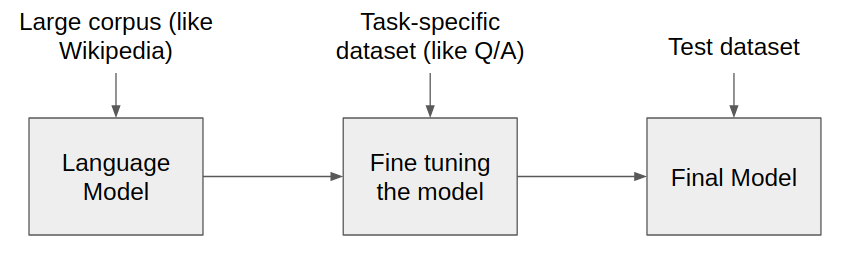
\includegraphics[scale=0.5]{lm.png}
\caption{ Language Model Pre-Training Workflow} %cite ganesh
\end{center}
\end{figure}

Language model pre-training are extremely effective for improving many natural language processing task. As the \textit{ULMfit} fine-tuning approach of Language-Model pre-training has showed. %cite Howard and Ruder.

\subsubsection{BERT Model}

\textbf{BERT}, which stands for \textbf{B}idirectional  \textbf{E}ncoder  \textbf{R}epresentations from  \textbf{T}ransformers is designed to pre-train deep bidirectional representations from unlabeled text by jointly condition on both left and right context in all layers. As a result, the pre-trained BERT model can be fine-tuned with just one additional output layer to create state-of-the-art models for a wide range of NLP tasks. %cite BERT

BERT is conceptually simple and empirically powerful. It obtains new state-of-the-art results on eleven natural language processing tasks, including pushing GLUE %cite GLUE
score to $80.5 \%$ , MultiNLI %cite multiNLI
accuracy to $86.7\%$, SQuAD v1.1 %cite SQUAD
question answering test F1 to 93.2  and SQuAD v2.0 %cite SQUAD
Test F1 to 83.1. %cite BERT

\subsection{Related Work}

IIT Bombay did some research on developing strategies  for Sentiment Analysis in Hindi.  In the paper they considered three approaches. The first to construct a classifier model for Hindi using a training corpus in Hindi. The second approach is to train a model on annotated English corpus and translate a Hindi document to English in order to use this model. The third approach involves using a majority-based classifier for Hindi SentiWordNet. The results of the research show that the first approach outperforms the others. %cite hindi sentiment analysis stratergy

In the paper titled BHAAV - A Text Corpus for emotion analysis from Hindi Stories, authors indtroduce the first and largest Hindi text corpus named BHAAV. The corpus consists of 20,304 sentences collected from 230 different short stores spanning across 18 genres. Each sentence has been annotated into one of the five emotion categories \{ \textit{anger, joy, suspense, sad, and neutral}\}. The paper also discuss challenges in the annotation of low resource language such as Hindi, and discuss the proposed corpus along with its possible uses. %cite Bhaav
My first try for this project was to source this corpus for training our model, but since we couldn't get permission for the dataset I decided to use the approach of BERT Model.
\clearpage
\section{Methodology and Implementation}

This section details the methodology and implementation details of the project. In this section the following details are described -  features of the dataset, preprocessing, and overall preparation and implementation methods used.

\subsection{Dataset}

After the initial failure to get the access to the BHAAV dataset %cite BHAAV
 , it was decide to find other resources for dataset. As Hindi is a low resource language this seemed to be a very difficult task at hand. Finally, I found a github repository %cite github repo.
 which had the dataset appropriate for sentiment analysis. The dataset here contains various tweets in Hindi along with corresponding label describing the emotional tone of the tweet. The categories of the label are \textit{negative}, \textit{neutral}, \textit{positive}. Figure \ref{dataset} shows some record in the dataset.
 
 \begin{figure}[H]
 \begin{center}
 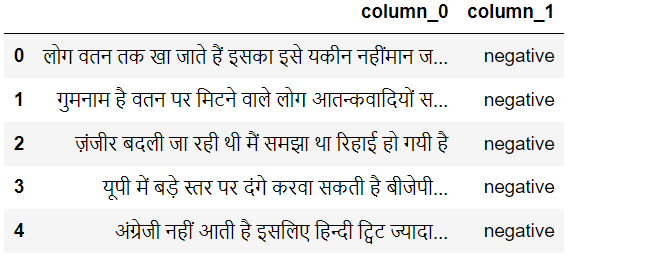
\includegraphics[scale=0.8]{dataset.png}
 \caption{ Subset of the dataset used in training the model.\label{dataset}}
 \end{center}
 \end{figure}
 
 The dataset contains \textit{\textbf{9077}} number of record. This dataset is then further divided into training, test and validation set. The total records in training set are \textit{\textbf{6353}} and the validation and test sets contains \textit{\textbf{1362}} and \textit{\textbf{1362}} records respectively. As, we can see \textit{\textbf{6353}} is comparatively a small number of records required to give a good accuracy on task like Sentiment Analysis. This is where transfer learning comes into play.
 
 \subsection{Preprocessing}
 
 There is not a lot of preprocessing done to the dataset. The first thing that is done is to encode the categorical data in label column as the model works on numerical values not text values. Label Encoding technique is used for this purpose. \textbf{Label Encoding} refers to converting the labels into numeric form so as to convert it into the machine-readable form. Machine learning algorithms can then decide in a better way on how those labels must be operated. It is an important pre-processing step for the structured dataset in supervised learning. %cite gfg
 We have three categories in our label data namely \textit{negative}, \textit{neutral}, and \textit{positive}. These will be converted to \textit{0} , \textit{1} and \textit{2} respectively.
 
 Secondly, for input we need to tokenize input as most NLP model are trained on tokens. For this we need to first make all the inputs of number of words . We do this by finding a cutoff number of words. For this we draw a histogram plot of all the inputs based on the total number of words they have and choose number of words that would satisfy most of the inputs. Figure \ref{plot} show the histogram distribution of input based on the total no. of words present in the piece of writing. And as we can see 35, is a good place to put our  cutoff. So that's what we've done. 
 
 \begin{figure}[H]
 \begin{center}
 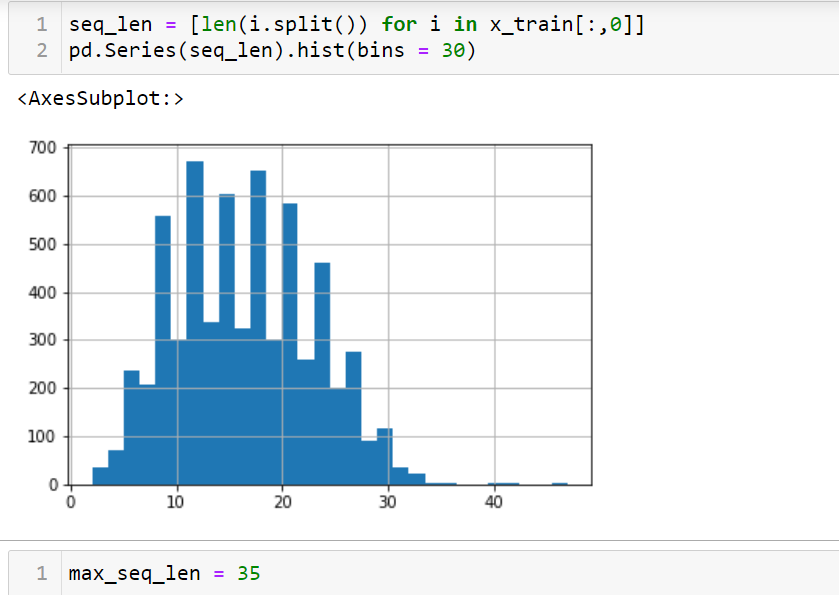
\includegraphics[scale=0.65]{maxlen.png}
 \caption{Histogram plot of the inputs based on the number of words\label{plot}}.
 \end{center}
 \end{figure}
 Then we have used to BERTTokenizerFast , a tokenizer pre-trained on multilingual dataset corpus. Tokenizer prepares our input in the following ways.
 \begin{itemize}
 \item{Tokenizing (splitting strings in sub-word token strings), converting tokens strings to ids and back, and encoding/decoding (i.e., tokenizing and converting to integers).} %cite BERT TOKENIZER

\item{Adding new tokens to the vocabulary in a way that is independent of the underlying structure (BPE, SentencePiece…).} %cite BERT TOKENIZER

\item{Managing special tokens (like mask, beginning-of-sentence, etc.): adding them, assigning them to attributes in the tokenizer for easy access and making sure they are not split during tokenization.} %cite BERT TOKENIZER
 \end{itemize}
 
 After the tokenization process is done we've feed these tokens as pytorch % cite pytorch
  tensors to be later transformed into pytorch DataClasses, which will be then used for training and validating in batches of fixed size. We have selected the batch size of 32.
  
  \subsection{Model}
  
  Our model has the following topology.
  \begin{itemize}
  \item{First our model has the BERT pre-trained multilingual model. To which the preprocessed input is passed to.}
  
  \item{Then the output of the BERT model is fed to the first layer of our model which contains 768 input, and 512 output Nodes. We have used the \textbf{Re}ctified \textbf{L}inear \textbf{U}nit activation function also called ReLU function at this layer. It is defined as $R(z) = max(0,z)$. It is usually a good first choice for an activation function based on some empirical evidences.}
  
  \item{Then we have used a dropout layer to which the output from first layer is passed to. This layer prevents from the problem of over fitting which is a very common issue in training models on complex datasets. The dropout layer helps us fix this issue by ignoring some of the input nodes. } %cite droupout layer article
  
  \item{The output from the dropout layer is passed to our output layer. The output layer consists of 512 input nodes (same as the output of first layer) and 3 output nodes. As we have three categories to classify our data, therefore we've used 3 output nodes. The activation function used in this layer is the softmax function. The standard softmax function: $ \sigma : \mathbb{R}^K \rightarrow [0,1]^K $ is defined as \large
  $\sigma(z)_i = \frac{e^{z_i}}{\sum_{j = 1} ^{ K} e^{z_j}}\  for\  i = 1, ... , K\  and\  z = (z1, ..., z_K) \in \mathbb{R}^K$. 
  \normalsize
  The softmax function is used to normalize the output of the  network to a probability distribution over predicted output classes. } %cite softmax wikipedia
  
  \end{itemize}
  
  We use \textit{sklearn.utils.class\_weight.compute\_class\_weight} library function to estimate initial weights for our model. This function estimates weights using heuristic inspired by  Logistic Regression in Rare Events Data, King, Zen, 2001. %cite this paper
  To calculate the loss we are using the cross entropy loss function. For a multiclass classification problem as we have, the cross entropy loss function can be defined as \large $- \sum_{c=1}^{M} y_{o,c} \ln(p_o,c)$.
  \normalsize
  
  \subsection{Training and Validation Process}
  
  \subsection{Testing Process}
  
  \section{Result and Conclusion}
  
  \section{Further work and improvement}
  
\clearpage
\printbibliography[heading=bibintoc]
\clearpage

\end{sloppypar}
\end{document}
